\chapter{Italics}

\index{Petrarch}
The first Italic type letter was derived, it is said, from the handwriting of Petrarch, and several admirable examples of the style, variously treated, have come down to us. As far as construction goes Italic is, theoretically, only the exact Roman form sloped, and with such changes as are necessitated by the sloping of the letters. Practically, however, it will be found that certain alterations in the outlines of the Roman letters must be made after giving them a slope in order to adapt them to their new requirements of inter-juxtaposition; and, by a reflex action, when words in Italic capitals are used in the same panel with upright Roman letters, certain variations must be made in the latter, such as accenting the Roman O in the same fashion as the Italic O is accented, an altered treatment of serifs, and other changes in detail.

\section{Typesetting italic text}
In \LaTeX\ three commands can be used to produce italic text: \verb+\textit, \emph+ and  \verb+\tt+. These are used as shown below:


\begin{verbatim}
The speaker is, \textit{ex officio}, the chairman.
The speaker is, \emph{ex officio}, the chairman.
The speaker is, {\tt ex officio}, the chairman.
\end{verbatim}

These will produce identical text as shown below,
\smallskip

\qquad  The speaker is, \textit{ex officio}, the chairman.

\qquad The speaker is, \emph{ex officio}, the chairman.

\qquad The speaker is, {\it ex officio}, the chairman.
\smallskip

The last one is the original \TeX\ command, but it is generally frowned upon to use it with \LaTeX\ despite the fact that Lamport has redefined it to be equaivalent to \verb+\textit+. Note that the last one needs to be enclosed in
braces unless you want your text from that point onwards to be typeset in italic font.

When typesetting mathematics, the \TeX\ engine typeset using italics unless specifically instructed to do otherwise:

\[\underbrace{\overbrace{a+b+c}^6
\cdot \overbrace{d+e+f}^9}
_\text{meaning of life} = 42\]

\begin{figure}
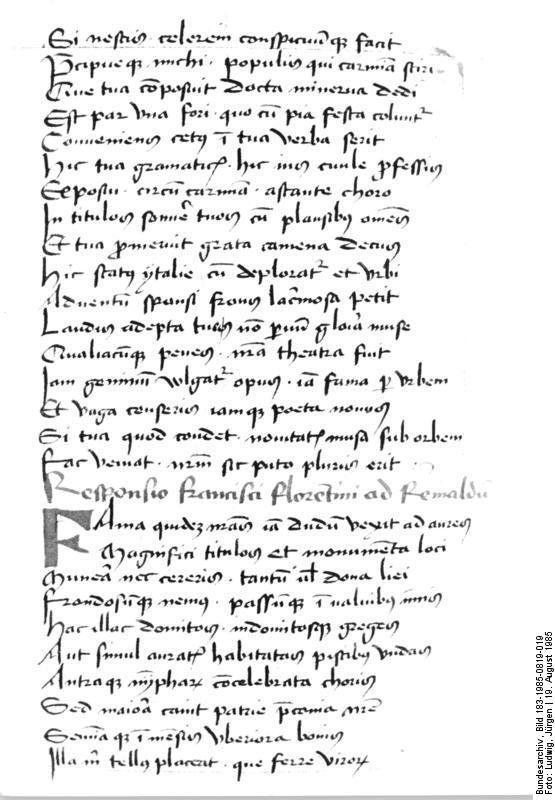
\includegraphics[width=0.8\textwidth]{petrarch}
\caption{Original lyrics by Petrarch, found in 1985 in Erfurt (source Wikipedia)}
\end{figure}

\chapter{RULES FOR THE USE OF ITALIC}

One very important principle should always be observed in the use of italic for emphasis. Emphasis should always be used sparingly. Make the words do their work. Do not try to supplement poverty of thought and weakness of expression by italics, capitals, and other marks of emphasis. Where there is too much emphasis attempted no emphasis is secured. This fault was much more common formerly than now.

The accompanying reproduction of a page from a book printed in 1690 (place not given, but probably London) illustrates several of the faulty uses of italics common at that time. An entire paragraph is italicized (quite unnecessarily) for emphasis. All proper names and adjectives derived from them are italicized where they occur in the regular text and printed in roman where they occur in italicized passages. Note the frequent capitalization for emphasis and especially the italic capital with roman lower-case in the first line of the second paragraph. This is a frequent usage in this particular book. In this book all quotations are printed in italic without quote marks. The paper, composition, and presswork of the book are very poor. It represents English printing in its worst period.

Moderation in the use of italics is so important that in many cases the compositor is justified in ignoring markings for italic in his copy where they are too profuse. The author is often surprised and disappointed at the appearance[7] of his proof when it comes back heavily italicized. Moreover the occurrence of many italics increases the cost of composition because of the greater labor involved.

\begin{enumerate}
\item  Italicize, subject to the caution just given, any words or phrases which it is desired to emphasize.

\item Foreign words and phrases incorporated into English sentences are sometimes italicized and sometimes not so distinguished. The deciding element in fixing the usage in these cases would seem to be the commonness and familiarity of the word or phrase. For example, the meaning of bona fide (Latin), menu (French), recto (Italian), or stein (German) are as well known as those of most English words. To all intents and purposes these words have been adopted into our language. On the other hand, jeu d'esprit (French) or inter alia (Latin) would probably not be immediately understood by the casual reader. Words of the first type should not be italicized. Words of the second type should be.

\item Do not italicize foreign titles preceding names of foreign institutions or places, streets, etc., the meaning or position of which in English would call for roman type.
        \begin{quote}
         \noindent Pere Ladeau; Freiherr von Schwenau; the Place de la Concorde; the Museo delle Terme.
       \end{quote}

\item In text matter use roman for the name of any author, but italicize the title of the work. This applies to books, including plays, essays, cycles of poems, and single poems of considerable length, usually printed separately, and not from the context understood to form parts of a larger volume; pamphlets, treatises, tracts, documents, and periodicals (including regularly appearing proceedings and transactions). In the case of newspapers and periodicals the [10] name of the place of publication should be italicized when it forms an integral part of the name, but do not under ordinary circumstances italicize the article \emph{the}.


\item The phrases \textit{prima facie} and \textit{ex officio} are sometimes used to qualify the nouns which follow, and sometimes used as adverbs. As qualifiers they are often printed in roman with the hyphen.

     \hspace*{1em} Prima-facie evidence.

     \hspace*{1em} An ex-officio member of all committees.


When used as adverbs they may be printed in italics without the hyphen.

\qquad The evidence is, \textit{prima facie}, convincing.

\qquad The speaker is, \textit{ex officio}, the chairman.

Names of ships, especially when they are taken from places, as in the United States Navy, are often italicized.

\qquad\qquad U.S.S. \textit{Philadelphia}, U.S.S. \textit{Alabama}.

\item  Italicize particular letters of the alphabet when referred to as such.

         We use \emph{a} much more frequently than \emph{q}.
\end{enumerate}



\subsubsection{The italic correction}

\begin{figure}[htbp]
\vspace*{1ex}
\centering
\fbox{\begin{minipage}{0.28\textwidth}
\rmfamily

{\noindent{\scalebox{3}{\color{gray!70}(fjordtl)}}}

\fbox{{{\scalebox{3}{\color{red}\textit{(fjordtl\/)}}}}}

\fbox{{{\scalebox{3}{\color{red}\textit{(fjordtl)}}}}}

{{\scalebox{3}{\color{red}$(fjordtl)$}}}
\end{minipage}}

\caption{Italic correction}
\end{figure}
